\documentclass{extbook}[14pt]
\usepackage{multicol, enumerate, enumitem, hyperref, color, soul, setspace, parskip, fancyhdr, amssymb, amsthm, amsmath, latexsym, units, mathtools}
\everymath{\displaystyle}
\usepackage[headsep=0.5cm,headheight=0cm, left=1 in,right= 1 in,top= 1 in,bottom= 1 in]{geometry}
\usepackage{dashrule}  % Package to use the command below to create lines between items
\newcommand{\litem}[1]{\item #1

\rule{\textwidth}{0.4pt}}
\pagestyle{fancy}
\lhead{}
\chead{Answer Key for Module12M Version ALL}
\rhead{}
\lfoot{1000-6427}
\cfoot{}
\rfoot{test}
\begin{document}
\textbf{This key should allow you to understand why you choose the option you did (beyond just getting a question right or wrong). \href{https://xronos.clas.ufl.edu/mac1105spring2020/courseDescriptionAndMisc/Exams/LearningFromResults}{More instructions on how to use this key can be found here}.}

\textbf{If you have a suggestion to make the keys better, \href{https://forms.gle/CZkbZmPbC9XALEE88}{please fill out the short survey here}.}

\textit{Note: This key is auto-generated and may contain issues and/or errors. The keys are reviewed after each exam to ensure grading is done accurately. If there are issues (like duplicate options), they are noted in the offline gradebook. The keys are a work-in-progress to give students as many resources to improve as possible.}

\rule{\textwidth}{0.4pt}

\begin{enumerate}\litem{
For the information provided below, construct a linear model that describes the total distance of the path, $D$, in terms of the time spent on a particular path \textit{if we know that all parts of the path are equal length}.

\begin{center}
    \textit{ A bicyclist is training for a race on a hilly path. Their bike keeps track of their speed at any time, but not the distance traveled. Their speed traveling up a hill is 3 mph, 8 mph when traveling down a hill, and 5 mph when traveling along a flat portion. }
\end{center}
The solution is \( \text{The model can be found with the information provided, but isn't options 1-3.} \).\begin{enumerate}[label=\Alph*.]
\textbf{Plausible alternative answers include:}The coefficient here is calculated as if you were trying to model the time on the total path.
The coefficient here is calculated by multiplying the speeds together rather than adding them.
This would be correct if we knew the time spent on each path was equal.
* This is the correct option. Since the paths are equal length and the bike can travel different speeds on each part, the time spent on each path is not equal! The model would be $3t_u + 8t_d +5t_f$, where $t_u$ is time traveling up, $t_d$ is time traveling down, and $t_f$ is time traveling on a flat portion.
If you chose this option, please contact the coordinator to discuss why you think we cannot model the situation.
\end{enumerate}

\textbf{General Comment:} Be sure you pay attention to the variable we are writing the model in terms of. To create the model with a single variable, we have to know that variable is the same throughout each path!
}
\litem{
For the information below, construct a linear model that describes the total time $T$ spent on the path in terms of the distance of a particular part of the path \textit{if we know that all parts of the path are equal length}.

\begin{center}
    \textit{ A bicyclist is training for a race on a hilly path. Their bike keeps track of their speed at any time, but not the distance traveled. Their speed traveling up a hill is 6 mph, 9 mph when traveling down a hill, and 7 mph when traveling along a flat portion. }
\end{center}
The solution is \( 0.421 D \).\begin{enumerate}[label=\Alph*.]
\textbf{Plausible alternative answers include:}The coefficient here is calculated as if you were trying to model the distance on the total path.
The coefficient here is calculated by multiplying the distances together rather than adding.
* This is the correct option.
Since we know all parts of the path are equal length, we can treat all distance variables as the same variable, $D$.
If you chose this option, please contact the coordinator to discuss why you think we cannot model the situation.
\end{enumerate}

\textbf{General Comment:} Be sure you pay attention to the variable we are writing the model in terms of. To create the model with a single variable, we have to know that variable is the same throughout each path!
}
\litem{
For the scenario below, use the model for the volume of a cylinder as $V = \pi r^2 h$.

\begin{center}
    \textit{ Pringles wants to add 34 \text{percent} more chips to their cylinder cans and minimize the design change of their cans. They've decided that the best way to minimize the design change is to increase the radius and height by the same percentage. What should this increase be? }
\end{center}
The solution is \( \text{About } 10 \text{ percent} \).\begin{enumerate}[label=\Alph*.]
\textbf{Plausible alternative answers include:}This corresponds to not solving for the increase properly.
* This is the correct option.
This corresponds to treating both radius and height as equal contributors and not solving correctly.
This corresponds to solving correctly but treating both radius and height as equal contributors to the volume.
If you chose this, please contact the coordinator to discus how you solved the problem.
\end{enumerate}

\textbf{General Comment:} Remember that when plugging the increases of values in, you need to treat it as that percentage above 100. For example, a 5 percent increase means 105 percent.
}
\litem{
Determine the appropriate model for the graph of points below.

\begin{center}
    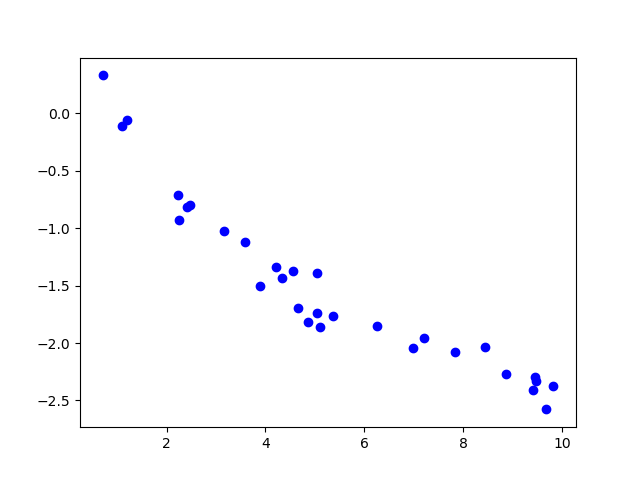
\includegraphics[width=0.5\textwidth]{../Figures/identifyModelGraph12CopyA.png}
\end{center}


The solution is \( \text{Non-linear Power model} \).\begin{enumerate}[label=\Alph*.]
\textbf{Plausible alternative answers include:}For this to be the correct option, we need to see a mostly straight line of points.
For this to be the correct option, we want an extremely slow change early, then a rapid change later.
For this to be the correct option, we need to see a polynomial or rational shape.
For this to be the correct option, we want a rapid change early, then an extremely slow change later.
For this to be the correct option, we want to see no pattern in the points.
\end{enumerate}

\textbf{General Comment:} This question is testing if you can associate the models with their graphical representation. If you are having trouble, go back to the corresponding Core module to learn about the specific function you are having trouble recognizing.
}
\litem{
For the scenario below, use the model for the volume of a cylinder as $V = \pi r^2 h$.

\begin{center}
    \textit{ Pringles wants to add 42 \text{percent} more chips to their cylinder cans and minimize the design change of their cans. They've decided that the best way to minimize the design change is to increase the radius and height by the same percentage. What should this increase be? }
\end{center}
The solution is \( \text{About } 12 \text{ percent} \).\begin{enumerate}[label=\Alph*.]
\textbf{Plausible alternative answers include:}This corresponds to solving correctly but treating both radius and height as equal contributors to the volume.
This corresponds to treating both radius and height as equal contributors and not solving correctly.
* This is the correct option.
This corresponds to not solving for the increase properly.
If you chose this, please contact the coordinator to discus how you solved the problem.
\end{enumerate}

\textbf{General Comment:} Remember that when plugging the increases of values in, you need to treat it as that percentage above 100. For example, a 5 percent increase means 105 percent.
}
\litem{
Determine the appropriate model for the graph of points below.

\begin{center}
    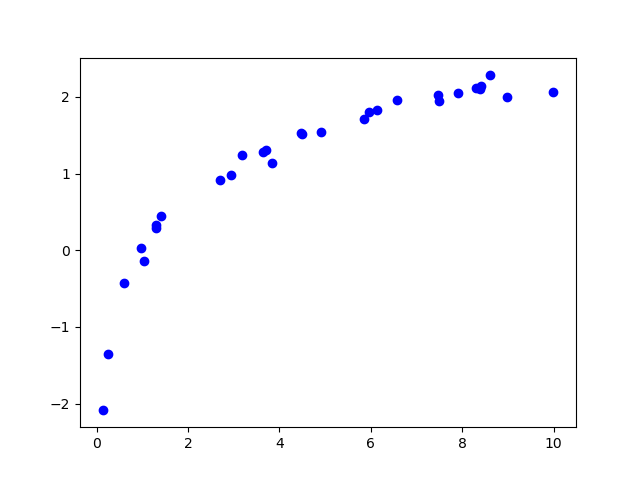
\includegraphics[width=0.5\textwidth]{../Figures/identifyModelGraph12A.png}
\end{center}


The solution is \( \text{Logarithmic model} \).\begin{enumerate}[label=\Alph*.]
\textbf{Plausible alternative answers include:}For this to be the correct option, we need to see a mostly straight line of points.
For this to be the correct option, we want an extremely slow change early, then a rapid change later.
For this to be the correct option, we want a rapid change early, then an extremely slow change later.
For this to be the correct option, we need to see a polynomial or rational shape.
For this to be the correct option, we want to see no pattern in the points.
\end{enumerate}

\textbf{General Comment:} This question is testing if you can associate the models with their graphical representation. If you are having trouble, go back to the corresponding Core module to learn about the specific function you are having trouble recognizing.
}
\litem{
Solve the modeling problem below, if possible.

\begin{center}
    \textit{ In CHM2045L, Brittany created a 29 liter 11 percent solution of chemical $\chi$ using two different solution percentages of chemical $\chi$. When she went to write her lab report, she realized she forgot to write the amount of each solution she used! If she remembers she used 7 percent and 23 percent solutions, what was the amount she used of the 7 percent solution? }
\end{center}
The solution is \( 21.75 liters \).\begin{enumerate}[label=\Alph*.]
\textbf{Plausible alternative answers include:}*This is the correct option.
This is the concentration of 23 percent solution.
This was a random value. If this was not a guess, contact the coordinator to talk about how you got this value.
This would be correct if Brittany used equal parts of each solution.
You may have chose this if you thought you needed to know how much of the second solution was used in the problem. Remember that the total minus the first solution would give you the second amount used.
\end{enumerate}

\textbf{General Comment:} Build the model exactly as you did in Module 9M. Then, solve for the volume you are looking for.
}
\litem{
Solve the modeling problem below, if possible.

\begin{center}
    \textit{ A new virus is spreading throughout the world. There were initially 5 many cases reported, but the number of confirmed cases has quadrupled every 5 days. How long will it be until there are at least 1000 confirmed cases? }
\end{center}
The solution is \( \text{About } 20 \text{ days} \).\begin{enumerate}[label=\Alph*.]
\textbf{Plausible alternative answers include:}You modeled the situation with $e$ as the base, but solved correctly otherwise.
* This is the correct option.
You modeled the situation correctly but did not apply the properties of log correctly.
You modeled the situation with $e$ as the base and did not apply the properties of log correctly.
If you chose this option, please contact the coordinator to discuss why you think this is the case.
\end{enumerate}

\textbf{General Comment:} Set up the model the same as in Module 11M. Then, plug in 1000 and solve for $d$ in your model.
}
\litem{
Solve the modeling problem below, if possible.

\begin{center}
    \textit{ In CHM2045L, Brittany created a 22 liter 17 percent solution of chemical $\chi$ using two different solution percentages of chemical $\chi$. When she went to write her lab report, she realized she forgot to write the amount of each solution she used! If she remembers she used 9 percent and 32 percent solutions, what was the amount she used of the 9 percent solution? }
\end{center}
The solution is \( 14.35 liters \).\begin{enumerate}[label=\Alph*.]
\textbf{Plausible alternative answers include:}*This is the correct option.
This was a random value. If this was not a guess, contact the coordinator to talk about how you got this value.
This would be correct if Brittany used equal parts of each solution.
This is the concentration of 32 percent solution.
You may have chose this if you thought you needed to know how much of the second solution was used in the problem. Remember that the total minus the first solution would give you the second amount used.
\end{enumerate}

\textbf{General Comment:} Build the model exactly as you did in Module 9M. Then, solve for the volume you are looking for.
}
\litem{
Solve the modeling problem below, if possible.

\begin{center}
    \textit{ A new virus is spreading throughout the world. There were initially 6 many cases reported, but the number of confirmed cases has quadrupled every 4 days. How long will it be until there are at least 10000 confirmed cases? }
\end{center}
The solution is \( \text{About } 22 \text{ days} \).\begin{enumerate}[label=\Alph*.]
\textbf{Plausible alternative answers include:}* This is the correct option.
You modeled the situation with $e$ as the base and did not apply the properties of log correctly.
You modeled the situation correctly but did not apply the properties of log correctly.
You modeled the situation with $e$ as the base, but solved correctly otherwise.
If you chose this option, please contact the coordinator to discuss why you think this is the case.
\end{enumerate}

\textbf{General Comment:} Set up the model the same as in Module 11M. Then, plug in 10000 and solve for $d$ in your model.
}
\litem{
The temperature of an object, $T$, in a different surrounding temperature $T_s$ will behave according to the formula $T(t) = Ae^{kt} + T_s$, where $t$ is minutes, $A$ is a constant, and k is a constant. Use this formula and the situation below to construct a model that describes the uranium's temperature, $T$, based on the amount of time t (in minutes) that have passed.

\begin{center}
    \textit{ Uranium is taken out of the reactor with a temperature of $100^{\circ}$ C and is placed into a $12^{\circ}$ C bath to cool. After 25 minutes, the uranium has cooled to $53^{\circ}$ C. }
\end{center}
The solution is \( \text{None of the above} \).\begin{enumerate}[label=\Alph*.]
\textbf{Plausible alternative answers include:}This uses $A$ as the initial temperature and solves for $k$ correctly.
This uses $A$ as the initial temperature and solves for $k$ incorrectly.
This uses $A$ as the bath temperature and solves for $k$ incorrectly.
This uses $A$ correctly and solves for $k$ incorrectly.
* This is the correct answer as $k = -0.03055$.
\end{enumerate}

\textbf{General Comment:} The initial temperature is when $t = 0$. Unlike power models, that means $A$ is not the initial temperature!
}
\litem{
For the scenario below, model the rate of vibration (cm/s) of the string in terms of the length of the string. Then determine the variation constant $k$ of the model (if possible). The constant should be in terms of cm and s.

\begin{center}
    \textit{ The rate of vibration of a string under constant tension varies based on the type of string and the length of the string. The rate of vibration of string $\omega$ increases as the quartic length of the string decreases. For example, when string $\omega$ is 5 mm long, the rate of vibration is 33 cm/s. }
\end{center}
The solution is \( k = 2.06 \).\begin{enumerate}[label=\Alph*.]
\textbf{Plausible alternative answers include:}* This is the correct option, which corresponds to the model $R = \frac{k}{l^{4}}$ AND converts from mm to cm.
This option uses the model $R = kl^{4}$ as if this is a direct variation AND does not convert from mm to cm so that the units match.
This option uses the correct model, $R = \frac{k}{l^{4}}$, but does not convert from mm to cm so that the units match.
This option uses the model $R = kl^{4}$ as if this is a direct variation.
Talk with the coordinator if you chose this option.
\end{enumerate}

\textbf{General Comment:} The most common mistake on this question is to not convert mm to cm! When modeling, you need to make sure all of the units for your variables are compatible.
}
\litem{
For the scenario below, use the model for the volume of a cylinder as $V = \pi r^2 h$.

\begin{center}
    \textit{ Pringles wants to add 49 \text{percent} more chips to their cylinder cans and minimize the design change of their cans. They've decided that the best way to minimize the design change is to increase the radius and height by the same percentage. What should this increase be? }
\end{center}
The solution is \( \text{About } 14 \text{ percent} \).\begin{enumerate}[label=\Alph*.]
\textbf{Plausible alternative answers include:}* This is the correct option.
This corresponds to treating both radius and height as equal contributors and not solving correctly.
This corresponds to not solving for the increase properly.
This corresponds to solving correctly but treating both radius and height as equal contributors to the volume.
If you chose this, please contact the coordinator to discus how you solved the problem.
\end{enumerate}

\textbf{General Comment:} Remember that when plugging the increases of values in, you need to treat it as that percentage above 100. For example, a 5 percent increase means 105 percent.
}
\litem{
Determine the appropriate model for the graph of points below.

\begin{center}
    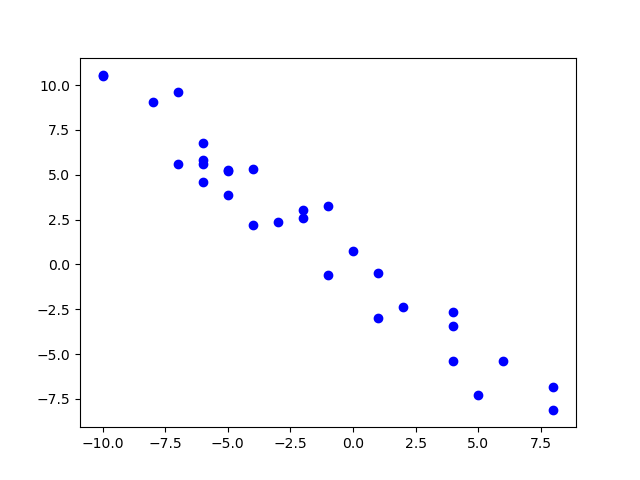
\includegraphics[width=0.5\textwidth]{../Figures/identifyModelGraph12CopyB.png}
\end{center}


The solution is \( \text{Linear model} \).\begin{enumerate}[label=\Alph*.]
\textbf{Plausible alternative answers include:}For this to be the correct option, we want an extremely slow change early, then a rapid change later.
For this to be the correct option, we need to see a polynomial or rational shape.
For this to be the correct option, we need to see a mostly straight line of points.
For this to be the correct option, we want a rapid change early, then an extremely slow change later.
For this to be the correct option, we want to see no pattern in the points.
\end{enumerate}

\textbf{General Comment:} This question is testing if you can associate the models with their graphical representation. If you are having trouble, go back to the corresponding Core module to learn about the specific function you are having trouble recognizing.
}
\litem{
For the scenario below, use the model for the volume of a cylinder as $V = \pi r^2 h$.

\begin{center}
    \textit{ Pringles wants to add 37 \text{percent} more chips to their cylinder cans and minimize the design change of their cans. They've decided that the best way to minimize the design change is to increase the radius and height by the same percentage. What should this increase be? }
\end{center}
The solution is \( \text{About } 11 \text{ percent} \).\begin{enumerate}[label=\Alph*.]
\textbf{Plausible alternative answers include:}This corresponds to treating both radius and height as equal contributors and not solving correctly.
This corresponds to not solving for the increase properly.
This corresponds to solving correctly but treating both radius and height as equal contributors to the volume.
* This is the correct option.
If you chose this, please contact the coordinator to discus how you solved the problem.
\end{enumerate}

\textbf{General Comment:} Remember that when plugging the increases of values in, you need to treat it as that percentage above 100. For example, a 5 percent increase means 105 percent.
}
\litem{
Determine the appropriate model for the graph of points below.

\begin{center}
    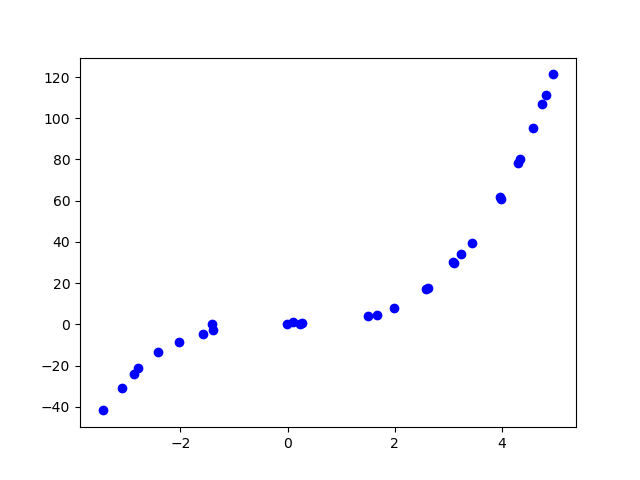
\includegraphics[width=0.5\textwidth]{../Figures/identifyModelGraph12B.png}
\end{center}


The solution is \( \text{Exponential model} \).\begin{enumerate}[label=\Alph*.]
\textbf{Plausible alternative answers include:}For this to be the correct option, we want a rapid change early, then an extremely slow change later.
For this to be the correct option, we need to see a mostly straight line of points.
For this to be the correct option, we want an extremely slow change early, then a rapid change later.
For this to be the correct option, we need to see a polynomial or rational shape.
For this to be the correct option, we want to see no pattern in the points.
\end{enumerate}

\textbf{General Comment:} This question is testing if you can associate the models with their graphical representation. If you are having trouble, go back to the corresponding Core module to learn about the specific function you are having trouble recognizing.
}
\litem{
Solve the modeling problem below, if possible.

\begin{center}
    \textit{ In CHM2045L, Brittany created a 20 liter 30 percent solution of chemical $\chi$ using two different solution percentages of chemical $\chi$. When she went to write her lab report, she realized she forgot to write the amount of each solution she used! If she remembers she used 19 percent and 46 percent solutions, what was the amount she used of the 46 percent solution? }
\end{center}
The solution is \( 8.15 liters \).\begin{enumerate}[label=\Alph*.]
\textbf{Plausible alternative answers include:}*This is the correct option.
This is the concentration of 19 percent solution.
This was a random value. If this was not a guess, contact the coordinator to talk about how you got this value.
This would be correct if Brittany used equal parts of each solution.
You may have chose this if you thought you needed to know how much of the second solution was used in the problem. Remember that the total minus the first solution would give you the second amount used.
\end{enumerate}

\textbf{General Comment:} Build the model exactly as you did in Module 9M. Then, solve for the volume you are looking for.
}
\litem{
Solve the modeling problem below, if possible.

\begin{center}
    \textit{ A new virus is spreading throughout the world. There were initially 6 many cases reported, but the number of confirmed cases has tripled every 5 days. How long will it be until there are at least 100000 confirmed cases? }
\end{center}
The solution is \( \text{About } 45 \text{ days} \).\begin{enumerate}[label=\Alph*.]
\textbf{Plausible alternative answers include:}You modeled the situation correctly but did not apply the properties of log correctly.
You modeled the situation with $e$ as the base and did not apply the properties of log correctly.
* This is the correct option.
You modeled the situation with $e$ as the base, but solved correctly otherwise.
If you chose this option, please contact the coordinator to discuss why you think this is the case.
\end{enumerate}

\textbf{General Comment:} Set up the model the same as in Module 11M. Then, plug in 100000 and solve for $d$ in your model.
}
\litem{
Solve the modeling problem below, if possible.

\begin{center}
    \textit{ In CHM2045L, Brittany created a 17 liter 26 percent solution of chemical $\chi$ using two different solution percentages of chemical $\chi$. When she went to write her lab report, she realized she forgot to write the amount of each solution she used! If she remembers she used 12 percent and 27 percent solutions, what was the amount she used of the 12 percent solution? }
\end{center}
The solution is \( 1.13 liters \).\begin{enumerate}[label=\Alph*.]
\textbf{Plausible alternative answers include:}*This is the correct option.
This is the concentration of 27 percent solution.
This was a random value. If this was not a guess, contact the coordinator to talk about how you got this value.
This would be correct if Brittany used equal parts of each solution.
You may have chose this if you thought you needed to know how much of the second solution was used in the problem. Remember that the total minus the first solution would give you the second amount used.
\end{enumerate}

\textbf{General Comment:} Build the model exactly as you did in Module 9M. Then, solve for the volume you are looking for.
}
\litem{
Solve the modeling problem below, if possible.

\begin{center}
    \textit{ A new virus is spreading throughout the world. There were initially 5 many cases reported, but the number of confirmed cases has quadrupled every 5 days. How long will it be until there are at least 1000 confirmed cases? }
\end{center}
The solution is \( \text{About } 20 \text{ days} \).\begin{enumerate}[label=\Alph*.]
\textbf{Plausible alternative answers include:}You modeled the situation correctly but did not apply the properties of log correctly.
You modeled the situation with $e$ as the base, but solved correctly otherwise.
You modeled the situation with $e$ as the base and did not apply the properties of log correctly.
* This is the correct option.
If you chose this option, please contact the coordinator to discuss why you think this is the case.
\end{enumerate}

\textbf{General Comment:} Set up the model the same as in Module 11M. Then, plug in 1000 and solve for $d$ in your model.
}
\litem{


\textbf{General Comment:} None
}
\litem{
Using the scenario below, model the situation using an exponential function and a base of $\frac{1}{2}$. Then, solve for the half-life of the element, rounding to the nearest day.

\begin{center}
    \textit{ The half-life of an element is the amount of time it takes for the element to decay to half of its initial starting amount. There is initially 974 grams of element $X$ and after 3 years there is 108 grams remaining. }
\end{center}
The solution is \( \text{About } 0 \text{ days} \).\begin{enumerate}[label=\Alph*.]
\textbf{Plausible alternative answers include:}This uses the correct model but a base of $e$ rather than $\frac{1}{2}$.
This uses the correct model but solves for the exponential constant incorrectly.
* This is the correct option.
This models half-life as a linear function.
Please contact the coordinator if you believe all the options above are incorrect.
\end{enumerate}

\textbf{General Comment:} The model should be $A(t) = A_0 (\frac{1}{2})^{kt}$, where $A(t)$ is the amount after $t$ years, $A_0$ is the initial amount, and $k$ is decay constant. To find the half-life, you need to solve for $k$ by using the amount after $x$ years, then solve for the time $t$ when $A = \frac{A_0}{2}$. Your answer would be in years, so convert to days.
}
\litem{
For the scenario below, use the model for the volume of a cylinder as $V = \pi r^2 h$.

\begin{center}
    \textit{ Pringles wants to add 43 \text{percent} more chips to their cylinder cans and minimize the design change of their cans. They've decided that the best way to minimize the design change is to increase the radius and height by the same percentage. What should this increase be? }
\end{center}
The solution is \( \text{About } 13 \text{ percent} \).\begin{enumerate}[label=\Alph*.]
\textbf{Plausible alternative answers include:}* This is the correct option.
This corresponds to not solving for the increase properly.
This corresponds to treating both radius and height as equal contributors and not solving correctly.
This corresponds to solving correctly but treating both radius and height as equal contributors to the volume.
If you chose this, please contact the coordinator to discus how you solved the problem.
\end{enumerate}

\textbf{General Comment:} Remember that when plugging the increases of values in, you need to treat it as that percentage above 100. For example, a 5 percent increase means 105 percent.
}
\litem{
Determine the appropriate model for the graph of points below.

\begin{center}
    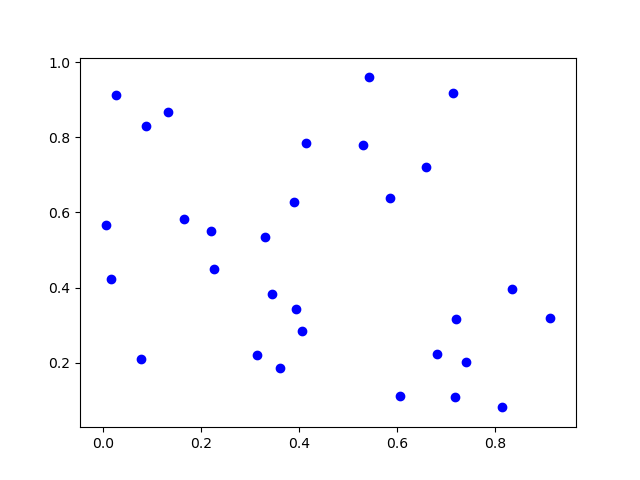
\includegraphics[width=0.5\textwidth]{../Figures/identifyModelGraph12CopyC.png}
\end{center}


The solution is \( \text{None of the above} \).\begin{enumerate}[label=\Alph*.]
\textbf{Plausible alternative answers include:}For this to be the correct option, we need to see a polynomial or rational shape.
For this to be the correct option, we want a rapid change early, then an extremely slow change later.
For this to be the correct option, we need to see a mostly straight line of points.
For this to be the correct option, we want an extremely slow change early, then a rapid change later.
For this to be the correct option, we want to see no pattern in the points.
\end{enumerate}

\textbf{General Comment:} This question is testing if you can associate the models with their graphical representation. If you are having trouble, go back to the corresponding Core module to learn about the specific function you are having trouble recognizing.
}
\litem{
For the scenario below, use the model for the volume of a cylinder as $V = \pi r^2 h$.

\begin{center}
    \textit{ Pringles wants to add 37 \text{percent} more chips to their cylinder cans and minimize the design change of their cans. They've decided that the best way to minimize the design change is to increase the radius and height by the same percentage. What should this increase be? }
\end{center}
The solution is \( \text{About } 11 \text{ percent} \).\begin{enumerate}[label=\Alph*.]
\textbf{Plausible alternative answers include:}This corresponds to solving correctly but treating both radius and height as equal contributors to the volume.
This corresponds to not solving for the increase properly.
This corresponds to treating both radius and height as equal contributors and not solving correctly.
* This is the correct option.
If you chose this, please contact the coordinator to discus how you solved the problem.
\end{enumerate}

\textbf{General Comment:} Remember that when plugging the increases of values in, you need to treat it as that percentage above 100. For example, a 5 percent increase means 105 percent.
}
\litem{
Determine the appropriate model for the graph of points below.

\begin{center}
    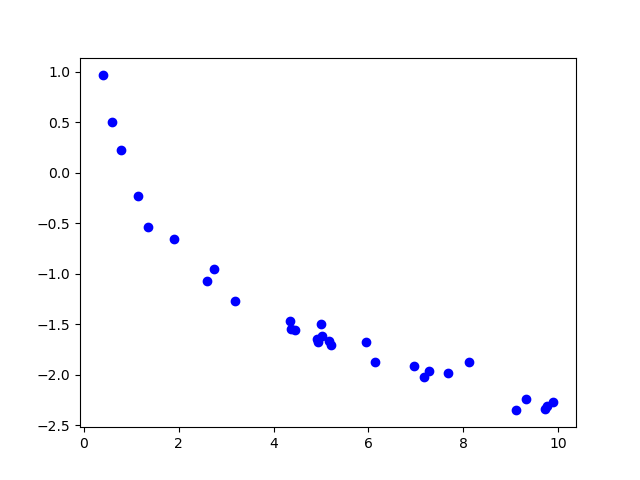
\includegraphics[width=0.5\textwidth]{../Figures/identifyModelGraph12C.png}
\end{center}


The solution is \( \text{Exponential model} \).\begin{enumerate}[label=\Alph*.]
\textbf{Plausible alternative answers include:}For this to be the correct option, we want a rapid change early, then an extremely slow change later.
For this to be the correct option, we want an extremely slow change early, then a rapid change later.
For this to be the correct option, we need to see a polynomial or rational shape.
For this to be the correct option, we need to see a mostly straight line of points.
For this to be the correct option, we want to see no pattern in the points.
\end{enumerate}

\textbf{General Comment:} This question is testing if you can associate the models with their graphical representation. If you are having trouble, go back to the corresponding Core module to learn about the specific function you are having trouble recognizing.
}
\litem{
Solve the modeling problem below, if possible.

\begin{center}
    \textit{ In CHM2045L, Brittany created a 18 liter 25 percent solution of chemical $\chi$ using two different solution percentages of chemical $\chi$. When she went to write her lab report, she realized she forgot to write the amount of each solution she used! If she remembers she used 15 percent and 43 percent solutions, what was the amount she used of the 43 percent solution? }
\end{center}
The solution is \( 6.43 liters \).\begin{enumerate}[label=\Alph*.]
\textbf{Plausible alternative answers include:}This would be correct if Brittany used equal parts of each solution.
This is the concentration of 15 percent solution.
This was a random value. If this was not a guess, contact the coordinator to talk about how you got this value.
*This is the correct option.
You may have chose this if you thought you needed to know how much of the second solution was used in the problem. Remember that the total minus the first solution would give you the second amount used.
\end{enumerate}

\textbf{General Comment:} Build the model exactly as you did in Module 9M. Then, solve for the volume you are looking for.
}
\litem{
Solve the modeling problem below, if possible.

\begin{center}
    \textit{ A new virus is spreading throughout the world. There were initially 8 many cases reported, but the number of confirmed cases has quadrupled every 5 days. How long will it be until there are at least 10000 confirmed cases? }
\end{center}
The solution is \( \text{About } 26 \text{ days} \).\begin{enumerate}[label=\Alph*.]
\textbf{Plausible alternative answers include:}You modeled the situation with $e$ as the base and did not apply the properties of log correctly.
* This is the correct option.
You modeled the situation with $e$ as the base, but solved correctly otherwise.
You modeled the situation correctly but did not apply the properties of log correctly.
If you chose this option, please contact the coordinator to discuss why you think this is the case.
\end{enumerate}

\textbf{General Comment:} Set up the model the same as in Module 11M. Then, plug in 10000 and solve for $d$ in your model.
}
\litem{
Solve the modeling problem below, if possible.

\begin{center}
    \textit{ In CHM2045L, Brittany created a 19 liter 19 percent solution of chemical $\chi$ using two different solution percentages of chemical $\chi$. When she went to write her lab report, she realized she forgot to write the amount of each solution she used! If she remembers she used 18 percent and 33 percent solutions, what was the amount she used of the 33 percent solution? }
\end{center}
The solution is \( 1.27 liters \).\begin{enumerate}[label=\Alph*.]
\textbf{Plausible alternative answers include:}*This is the correct option.
This is the concentration of 18 percent solution.
This would be correct if Brittany used equal parts of each solution.
This was a random value. If this was not a guess, contact the coordinator to talk about how you got this value.
You may have chose this if you thought you needed to know how much of the second solution was used in the problem. Remember that the total minus the first solution would give you the second amount used.
\end{enumerate}

\textbf{General Comment:} Build the model exactly as you did in Module 9M. Then, solve for the volume you are looking for.
}
\litem{
Solve the modeling problem below, if possible.

\begin{center}
    \textit{ A new virus is spreading throughout the world. There were initially 5 many cases reported, but the number of confirmed cases has tripled every 2 days. How long will it be until there are at least 10000 confirmed cases? }
\end{center}
The solution is \( \text{About } 14 \text{ days} \).\begin{enumerate}[label=\Alph*.]
\textbf{Plausible alternative answers include:}You modeled the situation with $e$ as the base, but solved correctly otherwise.
You modeled the situation with $e$ as the base and did not apply the properties of log correctly.
You modeled the situation correctly but did not apply the properties of log correctly.
* This is the correct option.
If you chose this option, please contact the coordinator to discuss why you think this is the case.
\end{enumerate}

\textbf{General Comment:} Set up the model the same as in Module 11M. Then, plug in 10000 and solve for $d$ in your model.
}
\end{enumerate}

\end{document}